\chapter{CRISP-DM}

\begin{description}
    \item[\Acl{crisp}] \marginnote{\acs{crisp}}
        Standardized process for data mining.
        \begin{figure}[ht]
            \centering
            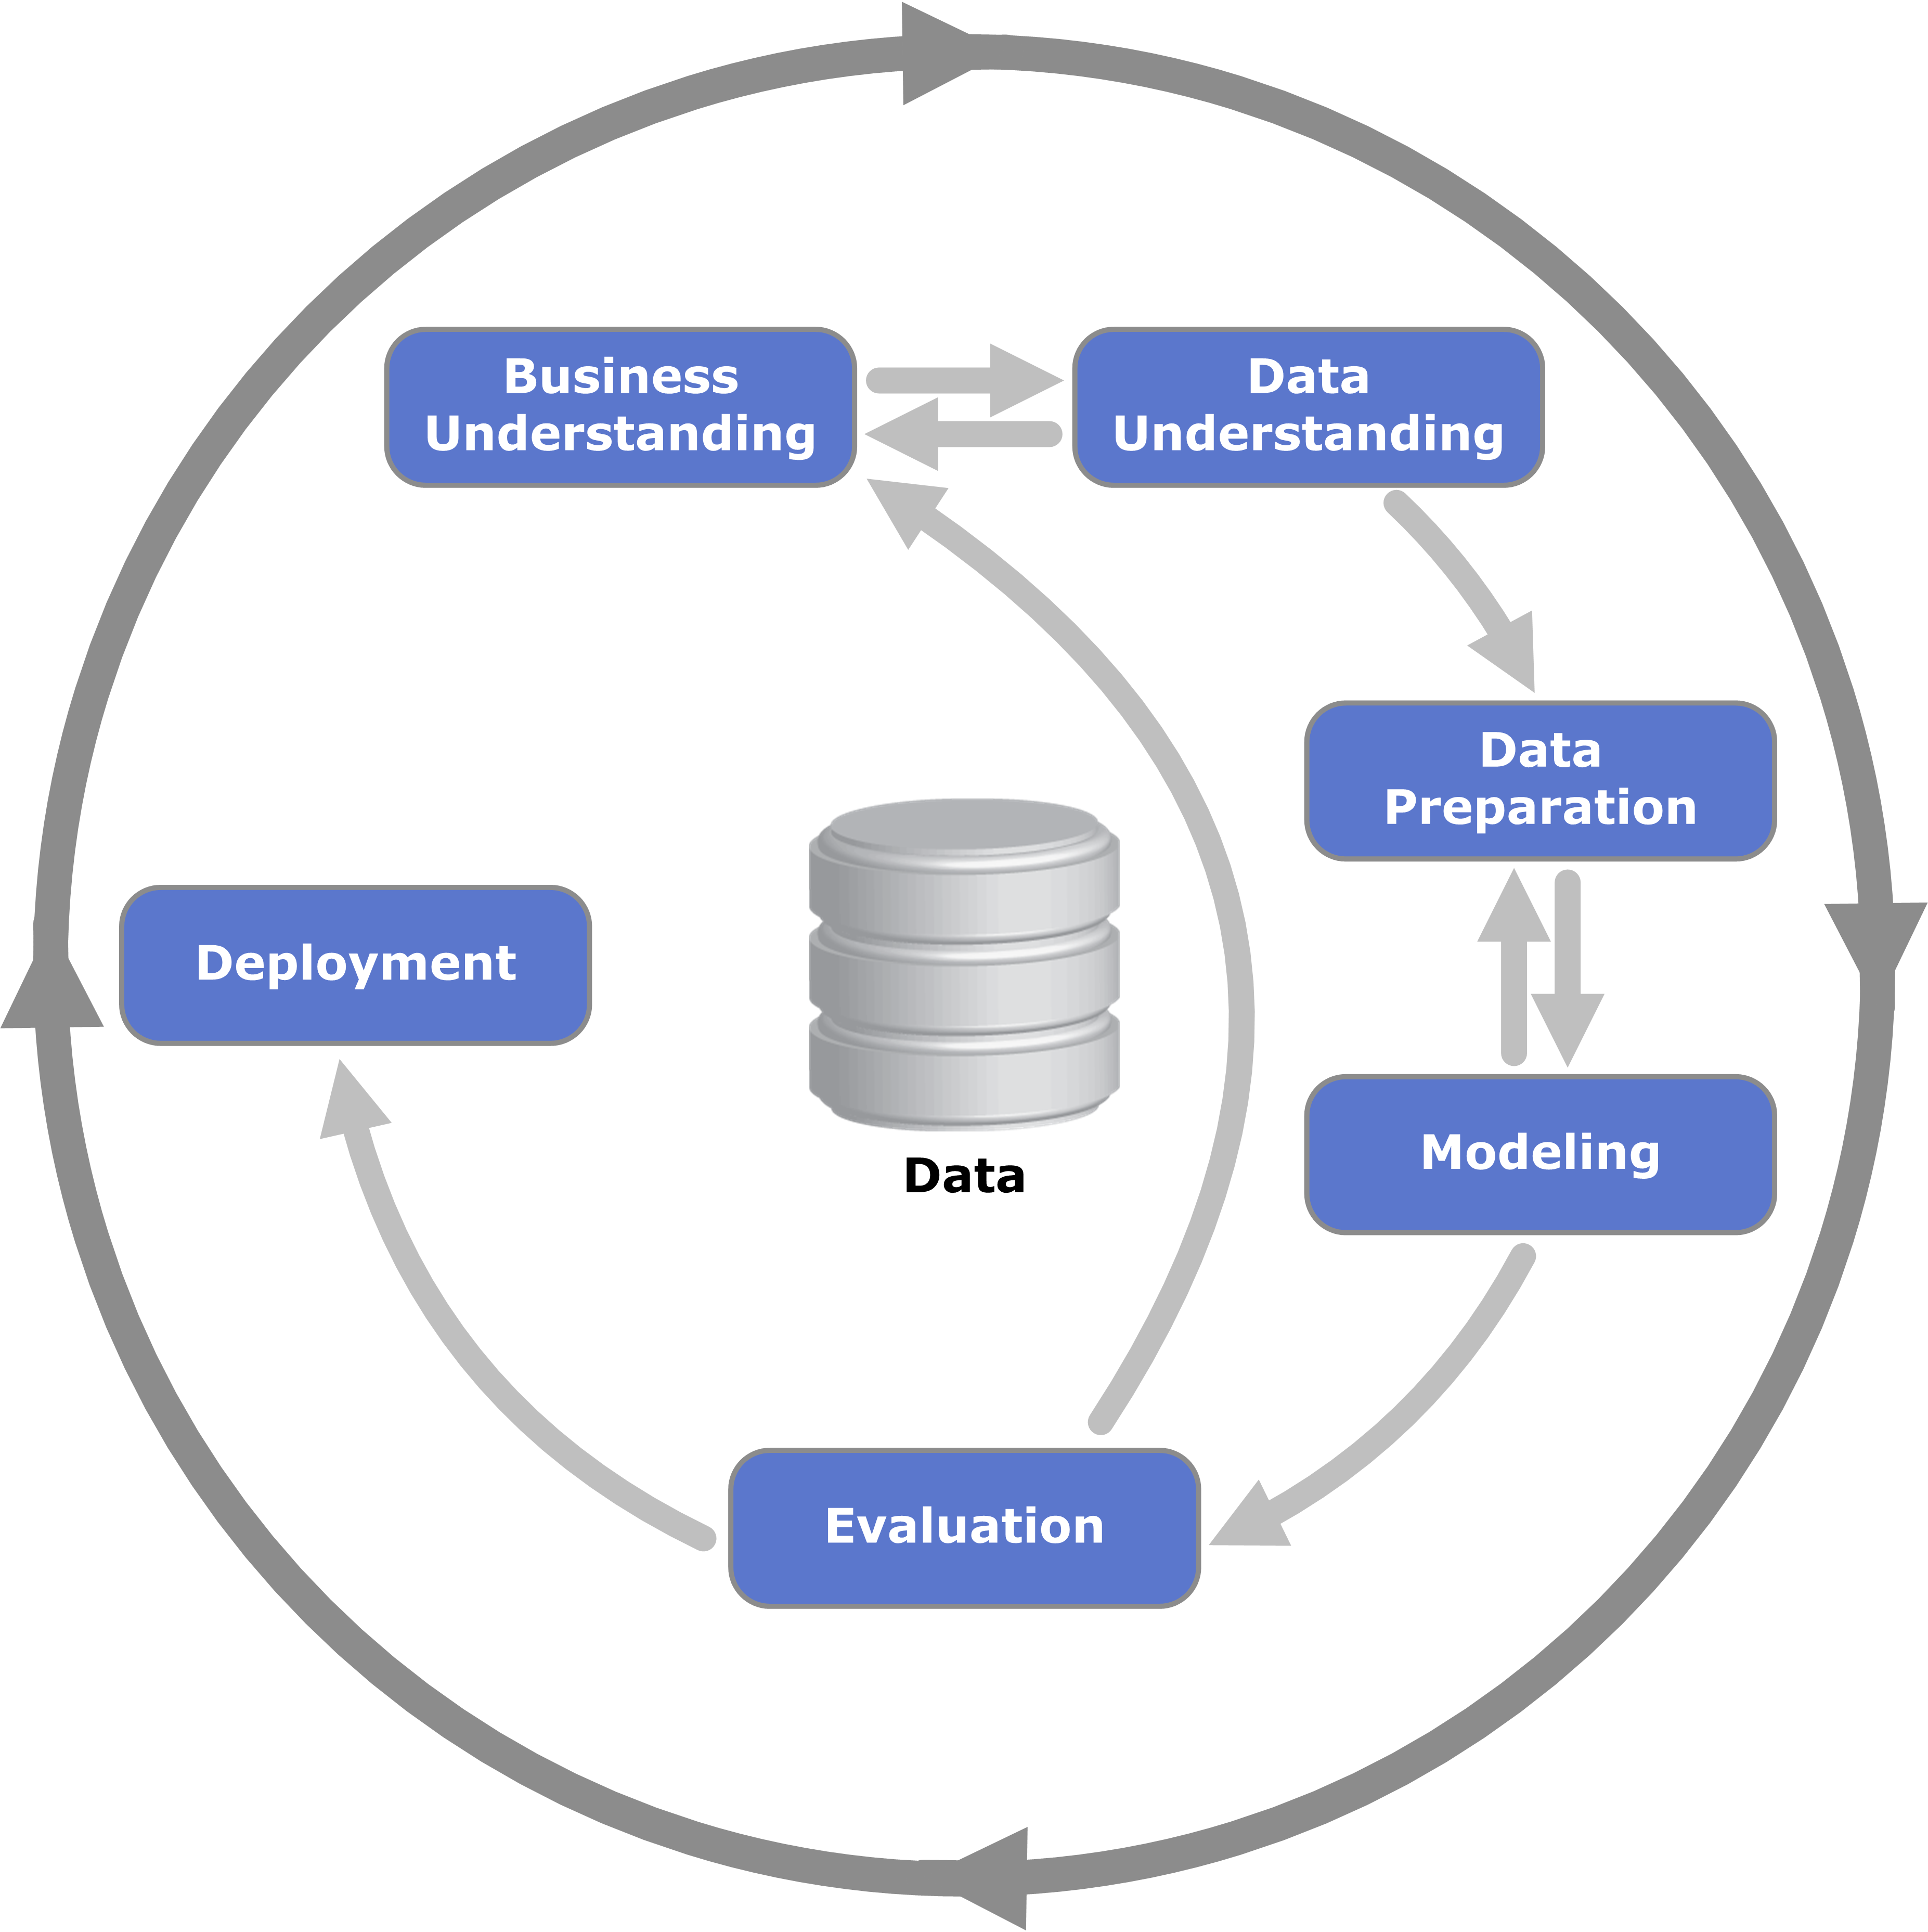
\includegraphics[width=0.45\textwidth]{img/crisp.png}
            \caption{\ac{crisp} workflow}
        \end{figure}
\end{description}


\section{Business understanding}
\begin{itemize}
    \item Determine the objective and the success criteria.
    \marginnote{Business understanding}
    \item Feasibility study.
    \item Produce a plan.
\end{itemize}

\section{Data understanding}
\begin{itemize}
    \item Determine the available (raw) data.
    \marginnote{Data understanding}
    \item Determine the cost of the data.
    \item Collect, describe, explore and verify data.
\end{itemize}

\section{Data preparation}
\begin{itemize}
    \item Data cleaning.
    \marginnote{Data preparation}
    \item Data transformations.
\end{itemize}

\section{Modeling}
\begin{itemize}
    \item Select modeling technique.
    \marginnote{Modeling}
    \item Build/train the model.
\end{itemize}

\section{Evaluation}
\begin{itemize}
    \item Evaluate results.
    \marginnote{Evaluation}
    \item Review process.
\end{itemize}

\section{Deployment}
\begin{itemize}
    \item Plan deployment.
    \marginnote{Deployment}
    \item Plan monitoring and maintenance.
    \item Final report and review.
\end{itemize}
